% !TeX root = ../main.tex
\usetikzlibrary{intersections, calc}

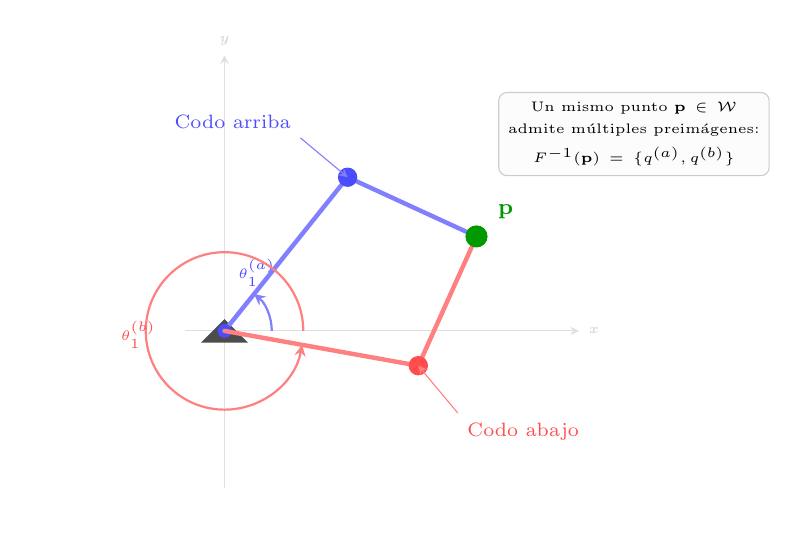
\begin{tikzpicture}[>=stealth, scale=1.0, every node/.style={font=\small}]

% 1. DEFINICIÓN DE PARÁMETROS
\coordinate (J0) at (0,0);           % Base
\coordinate (target) at (3.2, 1.2);  % Punto P objetivo
\def\lone{2.5}                       % Longitud eslabón 1
\def\ltwo{1.8}                       % Longitud eslabón 2

% 2. CÁLCULO AUTOMÁTICO DE LOS CODOS (Intersección de dos círculos)
\path[name path=c1] (J0) circle (\lone);
\path[name path=c2] (target) circle (\ltwo);
\path[name intersections={of=c1 and c2, by={J1up, J1down}}];

% --- Ejes y Base ---
\draw[->, gray!25] (-0.5,0) -- (4.5,0) node[right, font=\tiny, gray!40] {$x$};
\draw[->, gray!25] (0,-2) -- (0,3.5) node[above, font=\tiny, gray!40] {$y$};
\fill[black!70] (-0.3,-0.15) -- (0.3,-0.15) -- (0,0.15) -- cycle;

% =============================================
% CONFIGURACIÓN AZUL (Codo Arriba)
% =============================================
\draw[ultra thick, blue!50, line cap=round] (J0) -- (J1up) -- (target);
\fill[blue!70] (J0) circle (2.5pt);
\fill[blue!70] (J1up) circle (3.5pt);

% Etiqueta Codo Arriba (flecha TikZ nativa, sin triángulos manuales)
\draw[<-, blue!50, thin] (J1up) -- ++(-0.6, 0.5);
\node[blue!70, font=\scriptsize, anchor=south east] at ($(J1up)+(-0.6, 0.5)$) {Codo arriba};

% Arco θ₁(a) — radio pequeño, desde el eje x hasta el eslabón 1
% Ángulo calculado: atan2(y,x) de J1up relativo a J0
\pgfmathanglebetweenpoints{\pgfpointanchor{J0}{center}}{\pgfpointanchor{J1up}{center}}
\edef\angleUp{\pgfmathresult}
\draw[->, blue!50, thick] (0.6,0) arc (0:\angleUp:0.6);
\node[blue!70, font=\tiny, anchor=south] at ({0.5*cos(35)},{0.5*sin(35)+0.15}) {$\theta_1^{(a)}$};

% =============================================
% CONFIGURACIÓN ROJA (Codo Abajo)
% =============================================
\draw[ultra thick, red!50, line cap=round] (J0) -- (J1down) -- (target);
\fill[red!70] (J1down) circle (3.5pt);

% Etiqueta Codo Abajo (flecha TikZ nativa)
\draw[<-, red!50, thin] (J1down) -- ++(0.5, -0.6);
\node[red!70, font=\scriptsize, anchor=north west] at ($(J1down)+(0.5, -0.6)$) {Codo abajo};

% Arco θ₁(b) — radio más grande para no solapar con el azul
\pgfmathanglebetweenpoints{\pgfpointanchor{J0}{center}}{\pgfpointanchor{J1down}{center}}
\edef\angleDown{\pgfmathresult}
% Si el ángulo es negativo (codo abajo del eje x), dibujar hacia abajo
\draw[->, red!50, thick] (1.0,0) arc (0:\angleDown:1.0);
\node[red!70, font=\tiny] at ({1.1*cos(\angleDown/2)},{1.1*sin(\angleDown/2)-0.15}) {$\theta_1^{(b)}$};

% =============================================
% PUNTO P (Objetivo)
% =============================================
\fill[green!60!black] (target) circle (4pt);
\node[green!60!black, font=\footnotesize\bfseries, anchor=south west] at ($(target)+(0.15, 0.1)$) {$\mathbf{p}$};

% =============================================
% ANOTACIÓN LATERAL
% =============================================
\node[draw=black!20, rounded corners=3pt, fill=gray!2, 
      font=\tiny, text width=3.2cm, align=center] at (5.2, 2.5) {
    Un mismo punto $\mathbf{p} \in \mathcal{W}$\\[2pt]
    admite múltiples preimágenes:\\[3pt]
    $F^{-1}(\mathbf{p}) = \{q^{(a)}, q^{(b)}\}$
};

\end{tikzpicture}